%%%%%%%%%%%%%%%%%%%%%%%%%%%%%%%%%%%%%%%%%%%%%%%%%%%%%%%%%%%%%%%%%%%%%%%%%%%%%%%%%%
\begin{frame}[fragile]\frametitle{}
\begin{center}
{\Large sadhanpaad साधनपाद}
\end{center}
\end{frame}


%%%%%%%%%%%%%%%%%%%%%%%%%%%%%%%%%%%%%%%%%%%%%%%%%%%%%%%%%%%
\begin{frame}[fragile]\frametitle{Introduction}


	\begin{itemize}
	\item Sadhana in Sanskrit means `practice' and Sadhana Pada simply means, `the path of practice'. 	\item Here, in the second chapter of the Yoga Sutras, Patanjali explains the two paths or the two forms of Yoga: Kriya Yoga (क्रिया योग)and Ashtanga Yoga (Eightfold or Eight-limbed Yoga)
	\end{itemize}

\end{frame}

%%%%%%%%%%%%%%%%%%%%%%%%%%%%%%%%%%%%%%%%%%%%%%%%%%%%%%%%%%%
\begin{frame}[fragile]\frametitle{Kriya Yoga}


	\begin{itemize}
	\item The yoga of action, which consists of deliberate effort, a study of the self and traditional texts, and devotion. 
	\item The purpose of Kriya Yoga is to alleviate the causes of suffering and to attain Samadhi. 
	\item Kriya Yoga has three parts:
		\begin{itemize}
		\item Tapas – Endurance and Acceptance.
		\item Swadhyaaya – Self-awareness, and self-study.
		\item Ishwara Pranidhaana – Devotion to and love for the divine.
		\end{itemize}	
	\end{itemize}

\end{frame}

%%%%%%%%%%%%%%%%%%%%%%%%%%%%%%%%%%%%%%%%%%%%%%%%%%%%%%%%%%%
\begin{frame}[fragile]\frametitle{Ashtanga  Yoga}

A systematic and practical set of yogic knowledge divided into eight basic parts.

\begin{center}
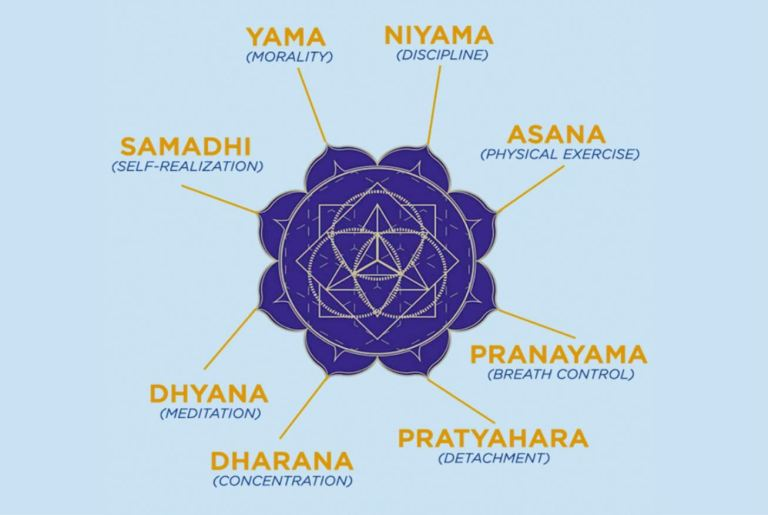
\includegraphics[width=0.6\linewidth,keepaspectratio]{images/yog22}
\end{center}

		\begin{itemize}
		\item Steps progression isn’t meant to be rigid. 
		\item For example, someone might begin the practice of an asana before they have mastered Niyama, still, they must follow the overall elements of the 8 limbs to have a wholesome growth.
		\end{itemize}
		
\end{frame}


%%%%%%%%%%%%%%%%%%%%%%%%%%%%%%%%%%%%%%%%%%%%%%%%%%%%%%%%%%%
\begin{frame}[fragile]\frametitle{Tapas}
\begin{sanskrit}
तपःस्वाध्यायेश्वरप्रणिधानानि क्रियायोगः॥१॥
\end{sanskrit}

	\begin{itemize}
	\item [HA]: Tapas (Austerity Or Sturdy Self-Discipline—Mental, Moral And Physical), Svadhyaya (Repetition Of Sacred Mattras Or Study Of Sacred Literature) And Isvara-Pranidhana (Complete Surrender To God) Are Kriya-Yoga (Yoga In The Form Of Action).
	\item [IT]: Austerity, self-study and resignation to Isvara constitute preliminary Yoga.
	\item [VH]: [BM]: The active performance of yoga involves ascetic practice, study of sacred lore, and dedication to the lord of Yoga.
	\item [SS]: Accepting pain as help for purification, study of spiritual books, and surrender to the Supreme Being constitute Yoga in practice.
	\item [SP]: Austerity, study, and the dedication of the fruits of one’s work to God: these are the preliminary steps toward yoga.
	\item [SV]: Mortification, study, and surrendering fruits of work to God are called Kriyâ-yoga. 
	\end{itemize}
\end{frame}

%%%%%%%%%%%%%%%%%%%%%%%%%%%%%%%%%%%%%%%%%%%%%%%%%%%%%%%%%%%
\begin{frame}[fragile]\frametitle{Klesas}
\begin{sanskrit}
समाधिभावनार्थः क्लेशतनूकरणार्थश्च॥२॥
\end{sanskrit}

	\begin{itemize}
	\item [HA]: For Bringing About Samadhi And Minimising The Klesas.
	\item [IT]: (Kriya-Yoga) is practiced for attenuating Klesas and bringing about Samadhi.
	\item [VH]: [BM]: It’s purpose is to cultivate pure contemplation and attenuate the forces of corruption.
	\item [SS]: They help us minimize obstackes and attain samadhi.
	\item [SP]: Thus we may cultivate the power of concentration and remove the obstacles to enlightenment which cause all our sufferings.
	\item [SV]: (It is for) the practice of Samadhi and minimising the pain-bearing obstructions. 
	\end{itemize}
\end{frame}



%%%%%%%%%%%%%%%%%%%%%%%%%%%%%%%%%%%%%%%%%%%%%%%%%%%%%%%%%%%
\begin{frame}[fragile]\frametitle{Avidya}
\begin{sanskrit}
अविद्यास्मितारागद्वेषाभिनिवेशाः क्लेशाः॥३॥
\end{sanskrit}

	\begin{itemize}
	\item [HA]: Avidya (Misapprehension About The Real Nature Of Things), Asmita (Egoism), Raga (Attachmant, Dvesa (Aversion) And Abhinivesa (Fear Of Death) Are The Five Klesas (Afflictions).
	\item [IT]: The lack of awareness of Reality, the sense of egoism or ‘I-am-ness’, attractions and repulsions towards objects and the strong desire for life are the great afflictions or causes of all miseries in life.
	\item [VH]: [BM]: The forces of corruption are ignorance, egoism. passion, hatred, and the will to live.
	\item [SS]: Ignorance, egoism, attachment, hatred, and clinging to bodily life are the five obstacles.
	\item [SP]: These obstacles—the causes of man’s sufferings—are ignorance, egoism, attachment, aversion, and the desire to cling to life.
	\item [SV]: The pain-bearing obstructions are — ignorance, egoism, attachment, aversion and clinging to life. 
	\end{itemize}
\end{frame}

%%%%%%%%%%%%%%%%%%%%%%%%%%%%%%%%%%%%%%%%%%%%%%%%%%%%%%%%%%%
\begin{frame}[fragile]\frametitle{Ignorance}
\begin{sanskrit}
अविद्याक्षेत्रमुत्तरेषां प्रसुप्ततनुविच्छिन्नोदाराणाम्॥४॥
\end{sanskrit}

	\begin{itemize}
	\item [HA]: Avidya Is The Breeding Ground For The Others Whether They Be Dormant, Attenuated, Interrupted Or Active.
	\item [IT]: Avidya is the source of those that are mentioned after it, whether they be in the dormant, attenuated, alternating or expanded condition.
	\item [VH]: [BM]: Ignorance is the field where the other forces of corruption develop, whether dormant, attenuated, intermittent, or active.
	\item [SS]: Ignorance is the field for the others mentioned after it, whether they be dormant, feeble, intercepted, or sustained.
	\item [SP]: Ignorance creates all the other obstacles. They may exist either in a potential or a vestigial form, or they may have been temporarily overcome or fully developed.
	\item [SV]: Ignorance is the productive field of all these that follow, whether they are dormant, attenuated, overpowered, or expanded. 
	\end{itemize}
\end{frame}


%%%%%%%%%%%%%%%%%%%%%%%%%%%%%%%%%%%%%%%%%%%%%%%%%%%%%%%%%%%
\begin{frame}[fragile]\frametitle{Transient}
\begin{sanskrit}
अनित्याशुचिदुःखानात्मसु नित्यशुचिसुखात्मख्यातिरविद्या॥५॥
\end{sanskrit}

	\begin{itemize}
	\item [HA]: Avidya Consists In Regarding A Transient Object As Everlasting, An Impure Object As Pure, Misery As Happiness And The Not-Self As Self.
	\item [IT]: Avidya is taking the non-eternal, impure, evil and non-Atman to be eternal, pure, good and Atman respectively.
	\item [VH]: [BM]: Ignorance is misperceiving permanance in transience, purity in impurity, pleasure in suffering, an essential self where there is no self.
	\item [SS]: Ignorance is regarding the impermanent as permanent, the impure as pure, the painful as pleasant, and the non-Self as Self.
	\item [SP]: To regard the noneternal as eternal, the impure as pure, the painful as pleasant and the non-Atman as the Atman-this is ignorance.
	\item [SV]: Ignorance is taking the non-eternal, the impure, the painful, and the non-Self, as the eternal, the pure, the happy, and the Atman or Self (respectively). 
	\end{itemize}
\end{frame}


%%%%%%%%%%%%%%%%%%%%%%%%%%%%%%%%%%%%%%%%%%%%%%%%%%%%%%%%%%%
\begin{frame}[fragile]\frametitle{Egoism}
\begin{sanskrit}
दृग्दर्शनशक्त्योरेकात्मतेवास्मिता॥६॥
\end{sanskrit}

	\begin{itemize}
	\item [HA]: Asmita Is Tantamount To The Identification Of Purusa Or Pure Consciousness With Buddhi.
	\item [IT]: Asmita is the identity of blending together, as it were, of the power of consciousness (Purusa) with the power of cognition (Buddhi).
	\item [VH]: [BM]: Egoism is ascribing a unified self to the organs and powers of perception, such as the eye and the power to see.
	\item [SS]: Egoism is the identification, as it were, of the power of the Seer (Purusha) with that of the instrument of seeing [body-mind].
	\item [SP]: To identify consciousness with that which merely reflects consciousness—this is egoism.
	\item [SV]: Egoism is the identification of the seer with the instrument of seeing. 
	\end{itemize}
\end{frame}



%%%%%%%%%%%%%%%%%%%%%%%%%%%%%%%%%%%%%%%%%%%%%%%%%%%%%%%%%%%
\begin{frame}[fragile]\frametitle{Attachment}
\begin{sanskrit}
सुखानुशयी रागः॥७॥
\end{sanskrit}

	\begin{itemize}
	\item [HA]: Attachment Is that (Modification) Which Follows Remembrance Of Pleasure.
	\item [IT]: That attraction, which accompanies pleasure, is Raga.
	\item [VH]: [BM]: Passion follows from attachment to pleasure.
	\item [SS]: Attachment is that which follows identification with pleasurable experiences.
	\item [SP]: Attachment is that which dwells upon pleasure.
	\item [SV]: Attachment is that which dwells on pleasure. 
	\end{itemize}
\end{frame}



%%%%%%%%%%%%%%%%%%%%%%%%%%%%%%%%%%%%%%%%%%%%%%%%%%%%%%%%%%%
\begin{frame}[fragile]\frametitle{Aversion}
\begin{sanskrit}
दुःखानुशयी द्वेषः॥८॥
\end{sanskrit}

	\begin{itemize}
	\item [HA]: Aversion Is That (Modification) Which Results From Misery.
	\item [IT]: That repulsion which accompanies pain is Dvesa.
	\item [VH]: [BM]: Hatred follows from attachment to suffering.
	\item [SS]: Aversion is that which follows identification with painful experiences.
	\item [SP]: Aversion is that which dwells upon pain.
	\item [SV]: Aversion is that which dwells on pain. 
	\end{itemize}
\end{frame}



%%%%%%%%%%%%%%%%%%%%%%%%%%%%%%%%%%%%%%%%%%%%%%%%%%%%%%%%%%%
\begin{frame}[fragile]\frametitle{Abhinivesa}
\begin{sanskrit}
स्वरसवाही विदुषोऽपि तथारूढो भिनिवेशः॥९॥
\end{sanskrit}

	\begin{itemize}
	\item [HA]: As In The Ignorant So In The Learned The Firmly Established Inborn Fear Of Annihilation Is The Affliction Called Abhinivesa.
	\item [IT]: Abhinivesa is the strong desire for life which dominates even the learned (or the wise).
	\item [VH]: [BM]: The will to live is instinctive and overwhelming, even for a learned sage.
	\item [SS]: Clinging to life, flowing by its own potency [due to past experience], exists even in the wise.
	\item [SP]: The desire to cling to life is inherent both in the ignorant and in the learned. This is because the mind retains impressions of the death experience from many previous incarnations.
	\item [SV]: Flowing through its own nature, and established even in the learned, is the clinging to life. 
	\end{itemize}
\end{frame}


%%%%%%%%%%%%%%%%%%%%%%%%%%%%%%%%%%%%%%%%%%%%%%%%%%%%%%%%%%%
\begin{frame}[fragile]\frametitle{Samskaras}
\begin{sanskrit}
ते प्रतिप्रसवहेयाः सूक्ष्माः॥१०॥
\end{sanskrit}

	\begin{itemize}
	\item [HA]: The Subtle Klesas Are Forsaken (i.e. Destroyed) By The Cessation Of Productivity (i.e. Disappearance) Of The Mind.
	\item [IT]: These, the subtle ones, can be reduced by resolving them backward into their origin.
	\item [VH]: 
	\item [BM]: The subtle forces of corruption can be escaped by reversing their course.
	\item [SS]: In subtle form, these obstacles can be destroyed by resolving them back into their primal cause [the ego].
	\item [SP]: When these obstacles have been reduced to a vestigial form, they can be destroyed by resolving the mind back into its primal cause.
	\item [SV]: The fine Samskaras are to be conquered by resolving them into their causal state. 
	\end{itemize}
\end{frame}


%%%%%%%%%%%%%%%%%%%%%%%%%%%%%%%%%%%%%%%%%%%%%%%%%%%%%%%%%%%
\begin{frame}[fragile]\frametitle{Subsistence}
\begin{sanskrit}
ध्यानहेयास्तद्वृत्तयः॥११॥
\end{sanskrit}

	\begin{itemize}
	\item [HA]: Their Means Of Subsistence Or Their Gross States Are Avoidable By Meditation.
	\item [IT]: Their active modifications are to be suppressed by meditation.
	\item [VH]: 
	\item [BM]: One can escape the turnings through meditation.
	\item [SS]: In the active state, they can be destroyed by meditation.
	\item [SP]: In their fully developed form, they can be overcome through meditation.
	\item [SV]: By meditation, their (gross) modifications are to be rejected. 
	\end{itemize}
\end{frame}


%%%%%%%%%%%%%%%%%%%%%%%%%%%%%%%%%%%%%%%%%%%%%%%%%%%%%%%%%%%
\begin{frame}[fragile]\frametitle{Karmasaya}
\begin{sanskrit}
क्लेशमूलः कर्माशयो दृष्टादृष्टजन्मवेदनीयः॥१२॥
\end{sanskrit}

	\begin{itemize}
	\item [HA]: Karmasaya Or Latent Impression of Action Based On Afflictions, Becomes Active In This Life Or In A Life To Come.
	\item [IT]: The resevoir of Karmas which are rooted in Klesas brings all kinds of experiences in the present and future lives.
	\item [VH]: 
	\item [BM]: Subliminal intention formed in actions, rooted in the forces of corruption, is realized in present or potential births.
	\item [SS]: The womb of karmas (actions and reactions) has its root in these obstacles, and the karmas bring experiences in the seen [present] or in the unseen [future] births.
	\item [SP]: A man’s latent tendencies have been created by his past thoughts and actions. These tendencies will bear fruits, both in this life and in lives to come.
	\item [SV]: The Receptacle of works has its root in these pain-bearing obstructions, and their experience is in this visible life, or in the unseen life. 
	\end{itemize}
\end{frame}


%%%%%%%%%%%%%%%%%%%%%%%%%%%%%%%%%%%%%%%%%%%%%%%%%%%%%%%%%%%
\begin{frame}[fragile]\frametitle{Fruits}
\begin{sanskrit}
सति मूले तद्विपाको जात्यायुर्भोगाः॥१३॥
\end{sanskrit}

	\begin{itemize}
	\item [HA]: As Long As Klesa Remains At The Root, Karmasaya Produces Three Consequences In The Form Of Birth, Span Of Life And Experience.
	\item [IT]: As long as the root is there it must ripen and result in lives of different class, length and experiences.
	\item [VH]: 
	\item [BM]: As long as this root exists, actions ripen into births, a term of life, and experience in the world.
	\item [SS]: With the existence of the root, there will be fruits also: namely, the births of different species of life, their life spans and experiences.
	\item [SP]: So long as the cause exists, it will bear fruits—such as rebirth, a long or a short life, and the experiences of pleasure and of pain.
	\item [SV]: The root being there, the fruition comes (in the form of) species, life, and expression of pleasure and pain. 
	\end{itemize}
\end{frame}


%%%%%%%%%%%%%%%%%%%%%%%%%%%%%%%%%%%%%%%%%%%%%%%%%%%%%%%%%%%
\begin{frame}[fragile]\frametitle{Experiences}
\begin{sanskrit}
ते ह्लादपरितापफलाः पुण्यापुण्यहेतुत्वात्॥१४॥
\end{sanskrit}

	\begin{itemize}
	\item [HA]: Because Of Virtue And Vice These (Birth, Span And Experience) Produce Pleasurable And Painful Experiences.
	\item [IT]: They have joy of sorrow for their fruit according as their cause is virtue of vice.
	\item [VH]: 
	\item [BM]: These actions bear joyful or sorrowful fruits according to the actor’s virtue or vice.
	\item [SS]: The karmas bear fruits of pleasure and pain caused by merit and demerit.
	\item [SP]: Experiences of pleasure and of pain are the fruits of merit and demerit, respectively.
	\item [SV]: They bear fruit as pleasure or pain, caused by virtue or vice. 
	\end{itemize}
\end{frame}


%%%%%%%%%%%%%%%%%%%%%%%%%%%%%%%%%%%%%%%%%%%%%%%%%%%%%%%%%%%
\begin{frame}[fragile]\frametitle{Discrimination}
\begin{sanskrit}
परिणामतापसंस्कारदुःखैर्गुणवृत्तिविरोधाच्च दुःखमेव सर्वं विवेकिनः॥१५॥
\end{sanskrit}

	\begin{itemize}
	\item [HA]: The Discriminating Persons Apprehend (By Analysis And Anticipation) All Worldly Objects As Sorrowful Because They Cause Suffering In Consequence, In Their Afflictive Experiences And In Their Latencies And Also Because Of The Contrary Nature Of The Gunas (Which Produces Changes All The Time).
	\item [IT]: To the people who have developed discrimination all is misery on account of the pains resulting from change, anxiety and tendencies, as also on account of the conflicts between the functioning of the Gunas and the Vrttis (of the mind).
	\item [VH]: 
	\item [BM]: All life is suffering for a man of discrimination, because of the sufferings inherant in change and its corrupting subliminal impression, and because of the way qualities of material nature turn against themselves.
	\item [SS]: To one of discrimination, everything is painful indeed, due to its consequences: the anxiety and fear over losing what is gained; the resulting impressions left in the mind to create renewed cravings; and the constant conflict among the three gunas, which control the mind.
	\item [SP]: But the man of spiritual discrimination regards al these experiences as painful. For even the enjoyment o present pleasure is painful, since we already fear it loss. Past pleasure is painful because renewed craving! arise from the impressions it has left upon the mind And how can any happiness be lasting if it depends only upon our moods? For these moods are constantly changing, as one or another of the ever-warring gunas seizes control of the mind.
	\item [SV]: To the discriminating, all is, as it were, painful on account of everything bringing pain, either in the consequences, or in apprehension, or in attitude caused by impressions, also on account of the counter action of qualities. 
	\end{itemize}
\end{frame}


%%%%%%%%%%%%%%%%%%%%%%%%%%%%%%%%%%%%%%%%%%%%%%%%%%%%%%%%%%%
\begin{frame}[fragile]\frametitle{Pain}
\begin{sanskrit}
हेयं दुःखमनागतम्॥१६॥
\end{sanskrit}

	\begin{itemize}
	\item [HA]: Pain Which Is Yet To Come Is To Be Discarded.
	\item [IT]: The misery which is not yet come can and is to be avoided.
	\item [VH]: 
	\item [BM]: Suffering that has not yet come can be escaped.
	\item [SS]: Pain that has not yet come is avoidable.
	\item [SP]: The pain which is yet to come may be avoided.
	\item [SV]: The misery which is not yet come is to be avoided. 
	\end{itemize}
\end{frame}


%%%%%%%%%%%%%%%%%%%%%%%%%%%%%%%%%%%%%%%%%%%%%%%%%%%%%%%%%%%
\begin{frame}[fragile]\frametitle{Uniting}
\begin{sanskrit}
द्रष्टृदृश्ययोः संयोगो हेयहेतुः॥१७॥
\end{sanskrit}

	\begin{itemize}
	\item [HA]: Uniting The Seer Or The Subject With The Seen Or The Object, Is The Cause Of That Which Has To Be Avoided.
	\item [IT]: The cause of that which is to be avoided is the union of the Seer and the Seen.
	\item [VH]: 
	\item [BM]: 
	\item [SS]: The cause of that avoidable pain is the union of the Seer (Purusha) and the seen (Prakriti, or Nature).
	\item [SP]: This pain is caused by false identification of the experiencer with the object of experience. It may be avoided.
	\item [SV]: The cause of that which is to be avoided is the junction of the seer and the seen. 
	\end{itemize}
\end{frame}

%%%%%%%%%%%%%%%%%%%%%%%%%%%%%%%%%%%%%%%%%%%%%%%%%%%%%%%%%%%
\begin{frame}[fragile]\frametitle{Seen}
\begin{sanskrit}
प्रकाशक्रियास्थितिशीलं भूतेन्द्रियात्मकं भोगापवर्गार्थं दृश्यम्॥१८॥
\end{sanskrit}

	\begin{itemize}
	\item [HA]: The Object Or Knowable Is By Nature Sentient, Mutable And Inert. It Exists In The Form Of The Elements And The Organs, And Serves The Purpose Of Experience And Emancipation.
	\item [IT]: The Seen (objective side of manifestation) consists of the elements and sense organs, is of the nature of cognition, activity and stability (Sattva, Rajas and Tamas) and has for its purpose providing the Purusa with) experience and liberation.
	\item [VH]: 
	\item [BM]: 
	\item [SS]: The seen is of the nature of the gunas: illumination, activity and inertia; and consists of the elements and sense organs, whose purpose is to provide both experiences and liberation to the Purusha.
	\item [SP]: The object of experience is composed of the three gunas—the principles of illumination (sattwa), activity (rajas) and inertia (tamas). From these, the whole universe has evolved together with the instruments of knowledge—such as the mind, senses, etc.—and the objects perceived—such as the physical elements. The universe exists in order that the experiencer may experience it, and thus become liberated.
	\item [SV]: The experienced is composed of elements and organs, is of the nature of illumination, action and intertia, and is for the purpose of experience and release (of the experiencer).

  
	\end{itemize}
\end{frame}


%%%%%%%%%%%%%%%%%%%%%%%%%%%%%%%%%%%%%%%%%%%%%%%%%%%%%%%%%%%
\begin{frame}[fragile]\frametitle{Gunas}
\begin{sanskrit}
विशेषाविशेषलिङ्गमात्रालिङ्गानि गुणपर्वाणि॥१९॥
\end{sanskrit}

	\begin{itemize}
	\item [HA]: Diversified (Visesa), Undiversified (Avisesa), Indicator-Only (Linga-Matra), And That Which Is Without Any Indication (Alinga), Are The States Of The Gunas.
	\item [IT]: The stages of the Gunas are the particular, the universal, the differentiated and the undifferentiated.
	\item [VH]: 
	\item [BM]: 
	\item [SS]: The stages of the gunas are specific, non-specific, defined and undefinable.
	\item [SP]: The gunas pass through four states—gross, subtle, primal and unevolved.
	\item [SV]: The states of the qualities are the defined, the undefined, the indicated only, and the signless. 
	\end{itemize}
\end{frame}

%%%%%%%%%%%%%%%%%%%%%%%%%%%%%%%%%%%%%%%%%%%%%%%%%%%%%%%%%%%
\begin{frame}[fragile]\frametitle{Absolute Knower}
\begin{sanskrit}
द्रष्टा दृशिमात्रः शुद्धोऽपि प्रत्ययानुपश्यः॥२०॥
\end{sanskrit}

	\begin{itemize}
	\item [HA]: The Seer Is Absolute Knower. Although Pure, Modifications (Of Buddhi) Are Witnessed By Him As An Onlooker.
	\item [IT]: The Seer is pure consciousness but though pure, appears to see through the mind.
	\item [VH]: 
	\item [BM]: 
	\item [SS]: The Seer is nothing but the power of seeing which, although pure, appears to see through the mind.
	\item [SP]: The Atman—the experiencer—is pure consciousness. It appears to take on the changing colors of the mind. In reality, it is unchangeable.
	\item [SV]: The seer is intelligence only, and though pure, seen through the colouring of the intellect. 
	\end{itemize}
\end{frame}


%%%%%%%%%%%%%%%%%%%%%%%%%%%%%%%%%%%%%%%%%%%%%%%%%%%%%%%%%%%
\begin{frame}[fragile]\frametitle{Purusa}
\begin{sanskrit}
तदर्थ एव दृश्यस्यात्मा॥२१॥
\end{sanskrit}

	\begin{itemize}
	\item [HA]: To Serve As Objective Field To Purusa Is The Essence Of Nature Of The Knowable.
	\item [IT]: The very being of the Seen is for his sake (i.e. Prakrti exists only for his sake).
	\item [VH]: 
	\item [BM]: 
	\item [SS]: The seen exists only for the sake of the Seer.
	\item [SP]: The object of experience exists only to serve the purpose of the Atman.
	\item [SV]: The nature of the experience is for him. 
	\end{itemize}
\end{frame}


%%%%%%%%%%%%%%%%%%%%%%%%%%%%%%%%%%%%%%%%%%%%%%%%%%%%%%%%%%%
\begin{frame}[fragile]\frametitle{Knowable}
\begin{sanskrit}
कृतार्थं प्रति नष्टमप्यनष्टं तदन्यसाधारणत्वात्॥२२॥
\end{sanskrit}

	\begin{itemize}
	\item [HA]: Although Ceasing To Exist In Relation To Him Whose Purpose Is Fulfilled The Knowable Does Not Cease To Exist On Account Of Being Of Use To Others.
	\item [IT]: Although it becomes non-existent for him whose purpose has been fulfilled it continues to exist for others on account of being common to others (besides him).
	\item [VH]: 
	\item [BM]: 
	\item [SS]: Although destroyed for him who has attained liberation, it [the seen] still exists for others, being common to them.
	\item [SP]: Though the object of experience becomes unreal to him who has reached the state of liberation, it remains real to all other beings.

[SV]: Though destroyed for him whose goal has been gained, yet is not destroyed, being common to others. 
	\end{itemize}
\end{frame}


%%%%%%%%%%%%%%%%%%%%%%%%%%%%%%%%%%%%%%%%%%%%%%%%%%%%%%%%%%%
\begin{frame}[fragile]\frametitle{Realisation}
\begin{sanskrit}
स्वस्वामिशक्त्योः स्वरूपोपलब्धिहेतुः संयोगः॥२३॥
\end{sanskrit}

	\begin{itemize}
	\item [HA]: Alliance Is The Means Of Realising The True Nature Of The Object Of the Knower And Of The Owner, The Knower (i.e. The Sort Of Alliance Which Contributes To The Realisation Of The Seer And The Seen Is This Relationship)
	\item [IT]: The purpose of the coming together of the Purusa and Prakrti is gaining by the Purusa of the awareness of his true nature and the unfoldment of powers inherent in him and the Prakrti.
	\item [VH]: 
	\item [BM]: 
	\item [SS]: The union of Owner (Purusha) and owned (Prakiti) causes the recognition of the nature and powers of them both.
	\item [SP]: The Atman—the experiencer—is identified with Prakriti—the object of experience–in order that the true nature of both Prakriti and Atman may be known.
	\item [SV]: Junction is the cause of the realisation of the nature of both the powers, the experienced and its Lord. 
	\end{itemize}
\end{frame}

%%%%%%%%%%%%%%%%%%%%%%%%%%%%%%%%%%%%%%%%%%%%%%%%%%%%%%%%%%%
\begin{frame}[fragile]\frametitle{Avidya}
\begin{sanskrit}
तस्य हेतुरविद्या॥२४॥
\end{sanskrit}

	\begin{itemize}
	\item [HA]: Avidya Or Nescience As Its Cause.
	\item [IT]: Its cause is the lack of awareness of his Real nature.
	\item [VH]: 
	\item [BM]: 
	\item [SS]: The cause of this union is ignorance.
	\item [SP]: This identification is caused by ignorance.
	\item [SV]: Ignorance is its cause. 
	\end{itemize}
\end{frame}

%%%%%%%%%%%%%%%%%%%%%%%%%%%%%%%%%%%%%%%%%%%%%%%%%%%%%%%%%%%
\begin{frame}[fragile]\frametitle{Dissociation}
\begin{sanskrit}
तदभावात् संयोगाभावो हानं तद् दृशेः कैवल्यम्॥२५॥
\end{sanskrit}

	\begin{itemize}
	\item [HA]: The Absence Of Alliance That Arises From Lack Of It Is The Freedom And That Is The State Of Liberation Of The Seer.
	\item [IT]: The dissociation of Purusa and Prakrti brought about by the dispersion of Avidya is the real remedy and that is the Liberation of the Seer.
	\item [VH]: 
	\item [BM]: 
	\item [SS]: Without this ignorance, no such union occurs. This is the independence of the Seer.
	\item [SP]: When ignorance has been destroyed, this identification ceases. Then bondage is at an end and the experiencer is indepedent and free.
	\item [SV]: There being absence of that (ignorance) there is absence of junction, which is the thingto-be-avoided; that is the independence of the seer. 
	\end{itemize}
\end{frame}

%%%%%%%%%%%%%%%%%%%%%%%%%%%%%%%%%%%%%%%%%%%%%%%%%%%%%%%%%%%
\begin{frame}[fragile]\frametitle{Discriminative Knowledge}
\begin{sanskrit}
विवेकख्यातिरविप्लवा हानोपायः॥२६॥
\end{sanskrit}

	\begin{itemize}
	\item [HA]: Clear And Distinct (Unimpaired) Discriminative Knowledge Is The Means Of Liberation.
	\item [IT]: The uninterrupted practice of the awareness of the Real is the means of dispersion (of Avidya).
	\item [VH]: 
	\item [BM]: 
	\item [SS]: Uninterrupted discriminative discernment is the method for its removal.
	\item [SP]: Ignorance is destroyed by awakening to knowledge of the Atman, until no trace of illusion remains.
	\item [SV]: The means of destruction of ignorance is unbroken practice of discrimination. 
	\end{itemize}
\end{frame}

%%%%%%%%%%%%%%%%%%%%%%%%%%%%%%%%%%%%%%%%%%%%%%%%%%%%%%%%%%%
\begin{frame}[fragile]\frametitle{Insight}
\begin{sanskrit}
तस्य सप्तधा प्रान्तभूमिः प्रज्ञा॥२७॥
\end{sanskrit}

	\begin{itemize}
	\item [HA]: Seven Kinds Of Ultimate Insight Come To Him (The Yogin Who Has Acquired Discriminative Enlightenment).
	\item [IT]: In his case the highest stage of Enlightenment is reached by seven stages.
	\item [VH]: 
	\item [BM]: 
	\item [SS]: One’s wisdom in the final stage is sevenfold. [One experiences the end of 1) desire to know anything more; 2) desire to stay away from any thing; 3) desire to gain anything new; 4) desire to do anything; 5) sorrow; 6) fear; 7) delusion.]
	\item [SP]: The experiencer gains this knowledge in seven stages, advancing toward the highest.
	\item [SV]: His knowledge is of the sevenfold highest ground. 
	\end{itemize}
\end{frame}


%%%%%%%%%%%%%%%%%%%%%%%%%%%%%%%%%%%%%%%%%%%%%%%%%%%%%%%%%%%
\begin{frame}[fragile]\frametitle{Impurities}
\begin{sanskrit}
योगाङ्गाऽनुष्ठानादशुद्धिक्षये ज्ञानदीप्तिराविवेकख्यातेः॥२८॥
\end{sanskrit}

	\begin{itemize}
	\item [HA]: Through The Practice Of The Different Accessories To Yoga When Impurities Are Destroyed, There Arises Enlightenment Culminating In Discriminative Enlightenment.
	\item [IT]: From the practice of the component exercises of Yoga, on the destruction of impurity, arises sprirtual illumination which develops into awareness of Reality.
	\item [VH]: 
	\item [BM]: 
	\item [SS]: By the practice of the limbs of Yoga, the impurities dwindle away and there dawns the light of wisdom, leading to discriminative discernment.
	\item [SP]: As soon as all impurities have been removed by the practice of spiritual disciplines—the “limbs” of yoga-a man’s spiritual vision opens to the light-giving knowledge of the Atman.
	\item [SV]: By the practice of the different parts of Yoga the impurities being destroyed knowledge becomes effulgent, up to discrimination. 
	\end{itemize}
\end{frame}

%%%%%%%%%%%%%%%%%%%%%%%%%%%%%%%%%%%%%%%%%%%%%%%%%%%%%%%%%%%
\begin{frame}[fragile]\frametitle{8 Limbs}
\begin{sanskrit}
यमनियमासनप्राणायामप्रत्याहारधारणाध्यानसमाधयोऽष्टावङ्गानि॥२९॥
\end{sanskrit}

	\begin{itemize}
	\item [HA]: Yama (Restraint), Niyama (Observance), Asana (Posture), Pranayama (Regulation Of Breath), Pratyahara (Withholding of Senses), Dharana (Fixity), Dhyana (Meditation) And Samadhi (Perfect Concentration) Are The Eight Means Of Attaining Yoga.
	\item [IT]: Self-restraints, fixed observances, posture, regulation of breath, abstraction, concentration, contemplation, trance are the eight parts (of the self-discipline of Yoga)
	\item [VH]: 
	\item [BM]: 
	\item [SS]:  Yama, Niyama, Asana, Pranayama, Pratyahara, Dharana, Dhyana, Sa
	\item [SP]: The eight limbs of yoga are: the various forms of abstention from evil-doing (yama), the various observances (niyamas), posture (asana), control of the prana (pranayams), withdrawal of the mind from sense objects (pratyahara), concentration (dharana), meditation (dhyana) and absorption in the Atman (samadhi).
	\item [SV]: Yama, Niyama, Asana, Pranayama, Pratyahara, Dharana, Dhyana, Samadhi, are the limbs of Yoga. 
	\end{itemize}
\end{frame}


%%%%%%%%%%%%%%%%%%%%%%%%%%%%%%%%%%%%%%%%%%%%%%%%%%%%%%%%%%%
\begin{frame}[fragile]\frametitle{Yama}
\begin{sanskrit}
अहिंसासत्यास्तेयब्रह्मचर्यापरिग्रहा यमाः॥३०॥
\end{sanskrit}

	\begin{itemize}
	\item [HA]: Ahimsa (Non-Injury), Satya (Truth), Asteya (Abstention From Stealing), Bramacharya (Continence), And Aparigraha (Abstinence From Avariciousness) Are The Five Yamas (Forms Of Restraint).
	\item [IT]: Vows of self-restraint comprise abstention from violence, falsehood, theft, incontinence and acquisitiveness.
	\item [VH]: 
	\item [BM]: 
	\item [SS]: Yama consists of non-violence, truthfulness, non-stealing, continence, and non-greed.
	\item [SP]: Yama is abstention from harming others, from falsehood, from theft, from incontinence, and from greed.
	\item [SV]: Non-killing, truthfulness, non-stealing, continence, and non-receiving, are called Yama. 
	\end{itemize}
\end{frame}


%%%%%%%%%%%%%%%%%%%%%%%%%%%%%%%%%%%%%%%%%%%%%%%%%%%%%%%%%%%
\begin{frame}[fragile]\frametitle{Yog}
\begin{sanskrit}
जातिदेशकालसमयानवच्छिन्नाः सार्वभौमा महाव्रतम्॥३१॥
\end{sanskrit}

	\begin{itemize}
	\item [HA]: However, (Become A) Great Vow When They Become Universal, Being Unrestricted By Any Consideration Of Class, Place Time Or Concept Of Duty.
	\item [IT]: These (the five vows) are not conditioned by class, place, time or occasion and extending to all stages constitute the Great Vow.
	\item [VH]: 
	\item [BM]: 
	\item [SS]: These Great Vows are universal, not limited by class, place, time or circumstance.
	\item [SP]: These forms of abstention are basic rules of conduct. They must be practised without any reservations as to time, place, purpose, or caste rules.
	\item [SV]: These, unbroken by time, place, purpose, and caste, are (universal) great vows. 
	\end{itemize}
\end{frame}



%%%%%%%%%%%%%%%%%%%%%%%%%%%%%%%%%%%%%%%%%%%%%%%%%%%%%%%%%%%
\begin{frame}[fragile]\frametitle{Niyama}
\begin{sanskrit}
शौचसंतोषतपःस्वाध्यायेश्वरप्रणिधानानि नियमाः॥३२॥
\end{sanskrit}

	\begin{itemize}
	\item [HA]: Cleanliness, Contentment, Austerity (Mental And Physical Discipline), Svadhyaya (Study Of Scriptures And Chanting Of Mantras) And Devotion To God Are The Niyamas.
	\item [IT]: Purity, contentment, austerity, self-study and self-surrender constitute observances.
	\item [VH]: 
	\item [BM]: 
	\item [SS]: Niyama consists of purity, contentment, accepting but not causing pain, study of spiritual books and worship of God [self-surrender].
	\item [SP]: The niyamas (observances) are purity, contentment, mortification, study and devotion to God.
	\item [SV]: Internal and external purification, contentment, mortification, study, and worship of God, are the Niyamas. 
	\end{itemize}
\end{frame}


%%%%%%%%%%%%%%%%%%%%%%%%%%%%%%%%%%%%%%%%%%%%%%%%%%%%%%%%%%%
\begin{frame}[fragile]\frametitle{Restraints}
\begin{sanskrit}
वितर्कबाधने प्रतिपक्षभावनम्॥३३॥
\end{sanskrit}

	\begin{itemize}
	\item [HA]: When These Restraints And Observances Are Inhibited By Perverse Thoughts The Opposites Should Be Thought Of.
	\item [IT]: When the mind is disturbed by improper thoughts constant pondering over the opposites (is the remedy).
	\item [VH]: 
	\item [BM]: 
	\item [SS]: When disturbed by negative thoughts, opposite [positive] ones should be thought of. This is pratipaksha bhavana.
	\item [SP]: To be free from thoughts that distract one from yoga, thoughts of an opposite kind must be cultivated.
	\item [SV]: To obstruct thoughts which are inimical to Yoga contrary thoughts will be brought. 
	\end{itemize}
\end{frame}



%%%%%%%%%%%%%%%%%%%%%%%%%%%%%%%%%%%%%%%%%%%%%%%%%%%%%%%%%%%
\begin{frame}[fragile]\frametitle{Perverse Thoughts}
\begin{sanskrit}
वितर्का हिंसादयः कृतकारितानुमोदिता लोभक्रोधमोहपूर्वका मृदुमध्याधिमात्रा दुःखाज्ञानानन्तफला इति प्रतिपक्षभावनम्॥३४॥
\end{sanskrit}

	\begin{itemize}
	\item [HA]: Actions Arising Out Of Perverse Thoughts Like Injury Etc. Are Either Performed By Oneself, Got Done By Another Or Approved ; Performed Either Through Anger Greed Or Delusion ; And Can Be Mild, Moderate Or Intense. That They Are The Causes Of Infinite Misery And Unending Ignorance Is The Contrary Thought.
	\item [IT]: As improper thoughts, emotions (and actions) such as those of violence etc., whether they are done (indulged in), caused to be done or abetted, whether caused by greed, anger or delusion, whether present in mild, medium or intense degree, result in endless pain and ignorance; so there is the necessity of pondering over the opposites.
	\item [VH]: 
	\item [BM]: 
	\item [SS]: When negative thoughts of acts such as violence, etc. are caused to be done or even approved of, whether incited by greed, anger or infatuation, whether indulged in with mild, medium or extreme intensity, they are based on ignorance and bring certain pain. Reflecting thus is also pratipaksha bhavana.
	\item [SP]: The obstacles to yoga—such as acts of violence and untruth— may be directly created or indirectly caused or approved, they may be motivated by greed, anger or self-interest, they may be small or moderate or great, but they never cease to result in pain and ignorance.
	\item [SV]: The obstructions to Yoga are killing etc., whether committed, caused, or approved; either through avarice, or anger, or ignorance; whether slight, middling, or great, and result is innumerable ignorances and miseries. This is (the method of) thinking the contrary. 
	\end{itemize}
\end{frame}

%%%%%%%%%%%%%%%%%%%%%%%%%%%%%%%%%%%%%%%%%%%%%%%%%%%%%%%%%%%
\begin{frame}[fragile]\frametitle{Yog}
\begin{sanskrit}
अहिंसाप्रतिष्ठायां तत्सन्निधौ वैरत्यागः॥३५॥
\end{sanskrit}

	\begin{itemize}
	\item [HA]: As The Yogin Becomes Established In Non-Injury, All Beings Coming Near Him Cease To Be Hostile.
	\item [IT]: On being firmly established in non-violence there is abandonment of hostility in (his) presence.
	\item [VH]: 
	\item [BM]: 
	\item [SS]: In the presence of one firmly established in non-violence, all hostilities cease.
	\item [SP]: When a man becomes steadfast in his abstention from harming others, then all living creatures will cease to feel enmity in his presence.
	\item [SV]: Non-killing being established, in his presence all emnities cease (in others). 
	\end{itemize}
\end{frame}


%%%%%%%%%%%%%%%%%%%%%%%%%%%%%%%%%%%%%%%%%%%%%%%%%%%%%%%%%%%
\begin{frame}[fragile]\frametitle{Truthfulness}
\begin{sanskrit}
सत्यप्रतिष्ठायां क्रियाफलाश्रयत्वम्॥३६॥
\end{sanskrit}

	\begin{itemize}
	\item [HA]: When Truthfulness Is Achieved The Words (Of The Yogin) Acquire The Power Of Making Them Fruitful.
	\item [IT]: On being firmly established in truthfulness fruit (of action) rests on action (of the Yogi) only.
	\item [VH]: 
	\item [BM]: 
	\item [SS]: To one established in truthfulness, actions and their results become subservient.
	\item [SP]: When a man becomes steadfast in his abstention from falsehood he gets the power of obtaining for himself and others the fruits of good deeds, without having to perform the deeds themselves.
	\item [SV]: By the establishment of truthfulness the Yogi gets the power of attaining for himself and others the fruits of work without the works. 
	\end{itemize}
\end{frame}


%%%%%%%%%%%%%%%%%%%%%%%%%%%%%%%%%%%%%%%%%%%%%%%%%%%%%%%%%%%
\begin{frame}[fragile]\frametitle{Non-Stealing}
\begin{sanskrit}
अस्तेयप्रतिष्ठायां सर्वरत्नोपस्थानम्॥३७॥
\end{sanskrit}

	\begin{itemize}
	\item [HA]: When Non-Stealing Is Established All Jewels Present Themselves.
	\item [IT]: On being firmly established in honesty all kinds of gems present themselves (before the Yogi).
	\item [VH]: 
	\item [BM]: 
	\item [SS]: To one established in non-stealing, all wealth comes.
	\item [SP]: When a man becomes steadfast in his abstention from theft, all wealth comes to him.
	\item [SV]: By the establishment of non-stealing all wealth comes to the Yogi. 
	\end{itemize}
\end{frame}


%%%%%%%%%%%%%%%%%%%%%%%%%%%%%%%%%%%%%%%%%%%%%%%%%%%%%%%%%%%
\begin{frame}[fragile]\frametitle{Virya}
\begin{sanskrit}
ब्रह्मचर्यप्रतिष्ठायां वीर्यलाभः॥३८॥
\end{sanskrit}

	\begin{itemize}
	\item [HA]: When Continence Is Established, Virya Is Acquired.
	\item [IT]: On being firmly established in sexual continence vigour (is) gained.
	\item [VH]: 
	\item [BM]: 
	\item [SS]: By one established in continence, vigor is gained.
	\item [SP]: When a man becomes steadfast in his abstention from incontinence, he acquires spiritual energy.
	\item [SV]: By the establishment of continence energy is gained. 
	\end{itemize}
\end{frame}


%%%%%%%%%%%%%%%%%%%%%%%%%%%%%%%%%%%%%%%%%%%%%%%%%%%%%%%%%%%
\begin{frame}[fragile]\frametitle{Perfection}
\begin{sanskrit}
अपरिग्रहस्थैर्ये जन्मकथंतासंबोधः॥३९॥
\end{sanskrit}

	\begin{itemize}
	\item [HA]: On Attaining Perfection In Non-Acceptance, Knowledge Of Past And Future Existences Arises.
	\item [IT]: Non-possessiveness being confirmed there arises knowledge of the ‘how’ and ‘wherefore’ of existence.
	\item [VH]: 
	\item [BM]: 
	\item [SS]: When non-greed is confirmed, a thorough illumination of the how and why of one’s birth comes.
	\item [SP]: When a man becomes steadfast in his abstention from greed, he gains knowledge of his past, present and future existences.
	\item [SV]: When he is fixed in non-receiving he gets the memory of past life. 
	\end{itemize}
\end{frame}



%%%%%%%%%%%%%%%%%%%%%%%%%%%%%%%%%%%%%%%%%%%%%%%%%%%%%%%%%%%
\begin{frame}[fragile]\frametitle{Purification}
\begin{sanskrit}
शौचात् स्वाङ्गजुगुप्सा परैरसंसर्गः॥४०॥
\end{sanskrit}

	\begin{itemize}
	\item [HA]: From The Practice Of Purification, Aversion Towards One’s Own Body Is Developed And Thus Aversion Extends To Contact With Other Bodies.
	\item [IT]: From physical purity (arises) disgust for one’s own body and disinclination to come in physical contact with others.
	\item [VH]: 
	\item [BM]: 
	\item [SS]: By purification arises disgust for one’s own body and for contact with other bodies.
	\item [SP]: As the result of purity, there arises indifference toward the body and disgust for physical intercourse with others.
	\item [SV]: Internal and external cleanliness being established, arises disgust for one’s own body, and non-intercourse with other bodies. 
	\end{itemize}
\end{frame}



%%%%%%%%%%%%%%%%%%%%%%%%%%%%%%%%%%%%%%%%%%%%%%%%%%%%%%%%%%%
\begin{frame}[fragile]\frametitle{Realisation}
\begin{sanskrit}
सत्त्वशुद्धिसौमनस्यैकाग्र्येन्द्रियजयात्मदर्शनयोग्यत्वानि च॥४१॥
\end{sanskrit}

	\begin{itemize}
	\item [HA]: Purification Of The Mind, Pleasantness Of Feeling, One-Pointedness, Subjugation Of The Senses And Ability For Self-Realisation Are Acquired.
	\item [IT]: From mental purity (arises) purity of Sattva, cheerful-mindedness, one-pointedness, control of the senses and fitness for the vision of the Self.
	\item [VH]: 
	\item [BM]: 
	\item [SS]: Moreover, one gains purity of sattva, cheerfulness of mind, one-pointedness, mastery over the senses, and fitness for Self-realization.
	\item [SP]: Moreover, one achieves purification of the heart, cheerfulness of mind, the power of concentration, control of the passions and fitness for vision of the Atman.
	\item [SV]: There also arises purification of the Sattva, cheerfulness of the mind, concentration, conquest of the organs, and fitness for the realisation of the Self. 
	\end{itemize}
\end{frame}


%%%%%%%%%%%%%%%%%%%%%%%%%%%%%%%%%%%%%%%%%%%%%%%%%%%%%%%%%%%
\begin{frame}[fragile]\frametitle{Contentment}
\begin{sanskrit}
संतोषादनुत्तमसुखलाभः॥४२॥
\end{sanskrit}

	\begin{itemize}
	\item [HA]: From Contentment Unsurpassed Happiness Is Gained.
	\item [IT]: Superlative happiness from contentment.
	\item [VH]: 
	\item [BM]: 
	\item [SS]: By contentment, supreme joy is gained.
	\item [SP]: As the result of contentment, one gains supreme happiness.
	\item [SV]: From contentment comes superlative happiness. 
	\end{itemize}
\end{frame}


%%%%%%%%%%%%%%%%%%%%%%%%%%%%%%%%%%%%%%%%%%%%%%%%%%%%%%%%%%%
\begin{frame}[fragile]\frametitle{Impurities}
\begin{sanskrit}
कायेन्द्रियसिद्धिरशुद्धिक्षयात्तपसः॥४३॥
\end{sanskrit}

	\begin{itemize}
	\item [HA]: Through Destruction Of Impurities, Practice Of Austerities Brings About Perfection Of The Body And The Organs.
	\item [IT]: Perfection of the sense-organs and body after destruction of impurity by austerities.
	\item [VH]: 
	\item [BM]: 
	\item [SS]: By austerity, impurities of body and senses are destroyed and occult powers gained.
	\item [SP]: As the result of mortification, impurities are removed. Then special powers come to the body and the sense organs.
	\item [SV]: The result of mortification is bringing powers to the organs and the body, by destroying the impurity. 
	\end{itemize}
\end{frame}


%%%%%%%%%%%%%%%%%%%%%%%%%%%%%%%%%%%%%%%%%%%%%%%%%%%%%%%%%%%
\begin{frame}[fragile]\frametitle{Mantras}
\begin{sanskrit}
स्वाध्यायादिष्टदेवतासंप्रयोगः॥४४॥
\end{sanskrit}

	\begin{itemize}
	\item [HA]: From Study And Repetition Of The Mantras Communion With The Desired Deity Is Established.
	\item [IT]: By (or from) self-study union with the desired deity.
	\item [VH]: 
	\item [BM]: 
	\item [SS]: By study of spiritual books comes communion with one’s chosen deity.
	\item [SP]: As the result of study, one obtains the vision of that aspect of God which one has chosen to worship.
	\item [SV]: By repetition of the mantram comes the realisation of the intended deity. 
	\end{itemize}
\end{frame}


%%%%%%%%%%%%%%%%%%%%%%%%%%%%%%%%%%%%%%%%%%%%%%%%%%%%%%%%%%%
\begin{frame}[fragile]\frametitle{Samadhi}
\begin{sanskrit}
समाधिसिद्धिरीश्वरप्रणिधानात्॥४५॥
\end{sanskrit}

	\begin{itemize}
	\item [HA]: From Devotion To God, Samadhi Is Attained.
	\item [IT]: Accomplishment of Samadhi from resignation to God.
	\item [VH]: 
	\item [BM]: 
	\item [SS]: By total surrender to God, samadhi is attained.
	\item [SP]: As the result of devotion to God, one achieves samadhi.
	\item [SV]: By sacrificing all to Isvara comes Samadhi. 
	\end{itemize}
\end{frame}


%%%%%%%%%%%%%%%%%%%%%%%%%%%%%%%%%%%%%%%%%%%%%%%%%%%%%%%%%%%
\begin{frame}[fragile]\frametitle{Asana}
\begin{sanskrit}
स्थिरसुखमासनम्॥४६॥
\end{sanskrit}

	\begin{itemize}
	\item [HA]: Motionless And Agreeable Form (Of Staying) Is Asana (Yogic Posture).
	\item [IT]: Posture (should be) steady and comfortable.
	\item [VH]: 
	\item [BM]: 
	\item [SS]: Asana is a steady, comfortable posture.
	\item [SP]: Posture (asana) is to be seated in a position which is firm but relaxed.
	\item [SV]: Posture is that which is firm and pleasant. 
	\end{itemize}
\end{frame}


%%%%%%%%%%%%%%%%%%%%%%%%%%%%%%%%%%%%%%%%%%%%%%%%%%%%%%%%%%%
\begin{frame}[fragile]\frametitle{Relaxation}
\begin{sanskrit}
प्रयत्नशैथिल्यानन्त्यसमापत्तिभ्याम्॥४७॥
\end{sanskrit}

	\begin{itemize}
	\item [HA]: By Relaxation Of Effort And Meditation On The Infinite (Asanas Are Perfected).
	\item [IT]: By relaxation of effort and meditation of the ‘ Endless ‘ (posture is attained)
	\item [VH]: 
	\item [BM]: 
	\item [SS]: By lessening the natural tendency for restlessness and by meditating on the infinite, posture is mastered.
	\item [SP]: Posture becomes firm and relaxed through control of the natural tendencies of the body, and through meditation on the infinite.
	\item [SV]: By slight effort and meditating on the unlimited (posture becomes firm and pleasant). 
	\end{itemize}
\end{frame}

%%%%%%%%%%%%%%%%%%%%%%%%%%%%%%%%%%%%%%%%%%%%%%%%%%%%%%%%%%%
\begin{frame}[fragile]\frametitle{Opposites}
\begin{sanskrit}
ततो द्वन्द्वानभिघातः॥४८॥
\end{sanskrit}

	\begin{itemize}
	\item [HA]: From That Arises Immunity From Dvandvas Or Opposite Conditions.
	\item [IT]: From that no assaults from the pairs of opposites.
	\item [VH]: 
	\item [BM]: 
	\item [SS]: Thereafter, one is undisturbed by the dualities.
	\item [SP]: Thereafter, one is no longer troubled by the dualities of sense-experience.
	\item [SV]: Seat being conquered, the dualities do not obstruct. 
	\end{itemize}
\end{frame}


%%%%%%%%%%%%%%%%%%%%%%%%%%%%%%%%%%%%%%%%%%%%%%%%%%%%%%%%%%%
\begin{frame}[fragile]\frametitle{Asana}
\begin{sanskrit}
तस्मिन् सति श्वासप्रश्वासयोर्गतिविच्छेदः प्राणायामः॥४९॥
\end{sanskrit}

	\begin{itemize}
	\item [HA]: That (Asana) Having Been Perfected, Regulation Of The Flow Of Inhalation And Exhalation Is Pranayama (Breath Control).
	\item [IT]: This having been (accomplished) Pranayama which is cessation of inspiration and expiration (follows).
	\item [VH]: That (asana-posture) being achieved, pranayama-breath regulation is interruption of the (normal) motion of inhalation and exhalation.
	\item [BM]: When the posture of yoga is steady, the breath is controlled by regulation of the course of exhalation and inhalation.
	\item [SS]: That [firm posture] being acquired, the movements of inhalation and exhalation should be controlled. This is pranayama. When this is [achieved], breath –control [which is] the cutting off of the flow of inhalation and exhalation [should be practiced
	\item [SP]: After mastering posture, one must practice control of the prana (pranayama) by stopping the motions of inhalation and exhalation.
	\item [SV]: Controlling the motion of the exhalation and the inhalation follows after this. 
	\end{itemize}
\end{frame}



%%%%%%%%%%%%%%%%%%%%%%%%%%%%%%%%%%%%%%%%%%%%%%%%%%%%%%%%%%%
\begin{frame}[fragile]\frametitle{Pranayama}
\begin{sanskrit}
बाह्याभ्यन्तरस्तम्भवृत्तिर्देशकालसंख्याभिः परिदृष्टो दीर्घसूक्ष्मः॥५०॥
\end{sanskrit}

	\begin{itemize}
	\item [HA]: That (Pranayama) Has External Operation (Vashya-Vrtti), Internal Operation (Abhyantara-Vrtti) And Supression (Stambha-Vrtti). These, Again, When Observed According To Space, Time, And Number Become Long And Subtle.
	\item [IT]: (It is in) external, internal or suppressed modifcation; is regulated by place, time and number, (and becomes progressively) prolonged and subtle.
	\item [VH]: (Pranayama has) external, internal or suspended modifications (which become) long and subtle, when observed by means of location (of breaths motion in the body), time (length of inhalation, exhalation and intervening spaces), and number.
	\item [BM]: The modification of breath in exhalation, inhalation, and retention is perceptible as deep and shallow breathing is regulated by where the breath is held, for how long, and for how many cycles.
	\item [SS]: The modifications of the life-breath are either external, internal or stationary. They are to be regulated by space, time and number and are either long or short.
	\item [SP]: The breath may be stopped externally, or internally, or checked in mid-motion, and regulated according to place, time and a fixed number of moments, so that the stoppage is either protracted or brief.
	\item [SV]: Its modifications are either external or internal, or motionless, regulated by place, time, and number, either long or short. 
	\end{itemize}
\end{frame}


%%%%%%%%%%%%%%%%%%%%%%%%%%%%%%%%%%%%%%%%%%%%%%%%%%%%%%%%%%%
\begin{frame}[fragile]\frametitle{Pranayama}
\begin{sanskrit}
बाह्याभ्यन्तरविषयाक्षेपी चतुर्थः॥५१॥
\end{sanskrit}

	\begin{itemize}
	\item [HA]: The Fourth Pranayama Transcends External And Internal Operations.
	\item [IT]: That Pranayama which goes beyond the sphere of internal and external is the fourth (variety).
	\item [VH]: The fourth (modification) transcends the reference to external and internal.
	\item [BM]: A fourth type of breath control goes beyond the range of exhalation and inhalation.
	\item [SS]: There is a fourth kind of pranayama that occurs during concentration on an internal or external object.
	\item [SP]: The fourth kind of pranayama is the stoppage of the breath which is caused by concentration upon external or internal objects.
	\item [SV]: The fourth is restraining the Prana by directing it either to the external or internal objects. 
	\end{itemize}
\end{frame}

%%%%%%%%%%%%%%%%%%%%%%%%%%%%%%%%%%%%%%%%%%%%%%%%%%%%%%%%%%%
\begin{frame}[fragile]\frametitle{Manifestation}
\begin{sanskrit}
ततः क्षीयते प्रकाशावरणम्॥५२॥
\end{sanskrit}

	\begin{itemize}
	\item [HA]: By That the Veil Over The Manifestation (Of Knowledge) Is Thinned.
	\item [IT]: From that is dissolved the covering of light.
	\item [VH]: Due to that, the covering of light is dispersed.
	\item [BM]: Then the cover over the light of truth dissolves.
	\item [SS]: As its result, the veil over the inner light is destroyed.
	\item [SP]: As the result of this, the covering of the Inner Light is removed.
	\item [SV]: From that, the covering to the light of the chitta is attenuated. 
	\end{itemize}
\end{frame}

%%%%%%%%%%%%%%%%%%%%%%%%%%%%%%%%%%%%%%%%%%%%%%%%%%%%%%%%%%%
\begin{frame}[fragile]\frametitle{Dharana}
\begin{sanskrit}
धारणासु च योग्यता मनसः॥५३॥
\end{sanskrit}

	\begin{itemize}
	\item [HA]: The Mind Acquires Fitness For Dharana.
	\item [IT]: And the fitness of the mind for concentration.
	\item [VH]: And readiness of the mind for dharana-focusings.
	\item [BM]: And the mind is fit for concentration.
	\item [SS]: And the mind becomes fit for concentration.
	\item [SP]: The mind gains the power of concentration (dharana).
	\item [SV]: The mind becomes fit for Dharana. 
	\end{itemize}
\end{frame}

%%%%%%%%%%%%%%%%%%%%%%%%%%%%%%%%%%%%%%%%%%%%%%%%%%%%%%%%%%%
\begin{frame}[fragile]\frametitle{Pratyahara}
\begin{sanskrit}
स्वविषयासंप्रयोगे चित्तस्य स्वरूपानुकार इवेन्द्रियाणां प्रत्याहारः॥५४॥
\end{sanskrit}

	\begin{itemize}
	\item [HA]: When Separated From Their Corresponding Objects, The Organs Follow, As It Were, The Nature Of The Mind, That Is Called Pratyahara (Restraining Of The Organs)
	\item [IT]: Pratyahara or abstraction is, as it were, the imitation by the senses of the mind by withdrawing themselves from their objects.
	\item [VH]: 
	\item [BM]: 
	\item [SS]: When the senses withdraw themselves from the objects and imitate, as it were, the nature of the mind-stuff, this is pratyahara.
	\item [SP]: When the mind is withdrawn from sense-objects, the sense-organs also withdraw themselves from their respective objects and thus are said to imitate the mind.
	\item [SV]: The drawing in of the organs is by their giving up their own objects and taking the form of the mind-stuff.
	\end{itemize}
\end{frame}

%%%%%%%%%%%%%%%%%%%%%%%%%%%%%%%%%%%%%%%%%%%%%%%%%%%%%%%%%%%
\begin{frame}[fragile]\frametitle{Control}
\begin{sanskrit}
ततः परमा वश्यतेन्द्रियाणाम्॥५५॥
\end{sanskrit}

	\begin{itemize}
	\item [HA]: That Brings Supreme Control Of The Organs.
	\item [IT]: Then follows the greatest mastery over the senses.
	\item [VH]: 
	\item [BM]: 
	\item [SS]: Then follows supreme mastery over the senses.
	\item [SP]: Thence arises complete mastery over the senses.
	\item [SV]: Thence arises supreme control of the organs. 
	\end{itemize}
\end{frame}

